% ------------------------------------------------------------------------------
% TYPO3 v9 LTS - What's New (English Version)
%
% @author	Michael Schams <schams.net>
% @license	Creative Commons BY-NC-SA 3.0
% @link		https://typo3.org/help/documentation/whats-new/
% @language	English
% ------------------------------------------------------------------------------

\section{Page-based URL Handling}
\begin{frame}[fragile]
	\frametitle{Page-based URL Handling}

	\begin{center}\huge{\color{typo3darkgrey}\textbf{Page-based URL Handling}}\end{center}
	\begin{center}\large{\textit{Speaking URLs "out of the box"}}\end{center}

\end{frame}

% ------------------------------------------------------------------------------
% #85947 - Page based URL handling

\begin{frame}[fragile]
	\frametitle{Page-based URL Handling}
	\framesubtitle{URL Segment}

	\begin{itemize}
		\item New field "URL Segment" has been added to page properties
		\item All links generated in the backend and frontend use this field, if set
		\item Languages are taken into account automatically
		\item No need for third-party extensions to generate "speaking URLs"
	\end{itemize}

	\begin{figure}
		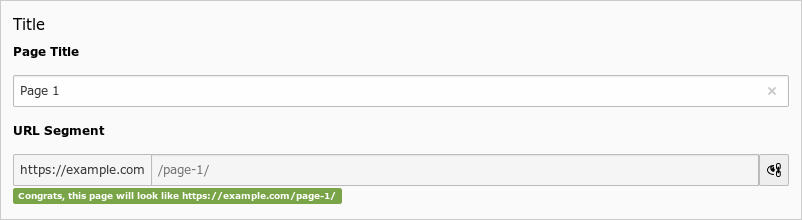
\includegraphics[width=0.8\linewidth]{PageBasedUrlHandling/UrlRouting.png}
	\end{figure}

%	\begin{figure}
%		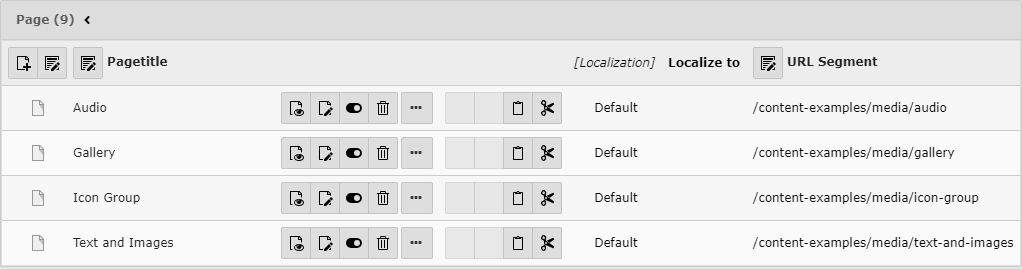
\includegraphics[width=0.8\linewidth]{PageBasedUrlHandling/85947-UrlSegments.png}
%	\end{figure}

\end{frame}

% ------------------------------------------------------------------------------
% #84729 - New TCA type "slug"

\begin{frame}[fragile]
	\frametitle{Page-based URL Handling}
	\framesubtitle{New TCA Field Type \texttt{slug}}

	% decrease font size for code listing
	\lstset{basicstyle=\smaller\ttfamily}

	\begin{itemize}
		\item New TCA field type \texttt{slug} has been added
		\item Define parts of a URL path to generate and resolve URLs

		\begin{lstlisting}
'type' => 'slug',
  'config' => [
    'generatorOptions' => [
      'fields' => ['title', 'nav_title'],
      'fieldSeparator' => '/',
      'prefixParentPageSlug' => true
    ]
    'fallbackCharacter' => '-',
    'eval' => 'uniqueInSite'
  ]
		\end{lstlisting}
	\end{itemize}

\end{frame}

% ------------------------------------------------------------------------------
% #86365 - Routing Enhancers and Aspects

\begin{frame}[fragile]
	\frametitle{Page-based URL Handling}
	\framesubtitle{Routing Enhancers and Aspects}

	% decrease font size for code listing
	\lstset{basicstyle=\smaller\ttfamily}

	\begin{itemize}
		\item Routes can be extended by "placeholders" to create URL paths such as:
			\smaller\texttt{/path-to/my-page/products/\{product-name\}}\normalsize
		\item This is done by "Enhancers" and "Aspects"
		\item TYPO3 v9 LTS supports the following enhancers out of the box:

			\begin{itemize}
				\item Simple Enhancer (enhancer type "Simple")
				\item Plugin Enhancer (enhancer type "Plugin")
				\item Extbase Plugin Enhancer (enhancer type "Extbase")
			\end{itemize}

		\item Configuration in file \texttt{config.yml} (no UI yet)
		\item Custom enhancers can be registered in \texttt{ext\_localconf.php}:

\begin{lstlisting}
$GLOBALS['TYPO3_CONF_VARS']['SYS']['routing']['CustomPlugin'] =
  \MyVendor\MyPackage\Routing\CustomEnhancer::class;
\end{lstlisting}
	\end{itemize}

\end{frame}

% ------------------------------------------------------------------------------
% #86160 - Add the possibility to use .html suffix in seo friendly URLs

\begin{frame}[fragile]
	\frametitle{Page-based URL Handling}
	\framesubtitle{Page Type Enhancer}

	% decrease font size for code listing
	\lstset{basicstyle=\smaller\ttfamily}

	\begin{itemize}
		\item The \texttt{PageTypeEnhancer} lets you configure pages by type,
			e.g. ones with the suffix \texttt{.html}
		\item The suffix gets added at the very end of a URL by using the
			\texttt{StaticValueMapper}
		\item Configuration example:

\begin{lstlisting}
routeEnhancers:
  PageType:
    type: PageType default: ''
	map:
	  '.html': 1
	  'menu.json': 13
\end{lstlisting}

	\end{itemize}

\end{frame}

% ------------------------------------------------------------------------------
